\documentclass{sig-alt-full}

\usepackage{graphicx}
\usepackage{url}

\begin{document}

\newcommand{\imp}[1]{{\small{\sf #1}}}
\newcommand{\stereotype}[1]{$<<${\small{\sf #1}}$>>$}

% --- Author Metadata here ---
\conferenceinfo{FOSD'10,}{October 13, 2010, Eindhoven (The Netherlands)}
\CopyrightYear{2010} \crdata{...}
% --- End of Author Metadata ---

\title{C\# Partial Classes as a Mechanisms to Implement Feature-Oriented Designs: An Exploratory Study\thanks{This work has been supported by the Spanish Ministry Project TIN2008-01942/TIN, the EC STREP Project AMPLE IST-033710, and the Junta de Andaluc{\'i}a regional project FarmWare TIC-5231.}}

\numberofauthors{3}

\author{
\alignauthor Elio L�pez \\
       \affaddr{Dpto. Lenguajes y Ciencias de la Computaci{\'o}n}\\
       \affaddr{Universidad de M{\'a}laga (Spain)}\\
       \email{ealopezs@gmail.com}
\alignauthor Pablo S{\'a}nchez \\
       \affaddr{Dpto. Matem{\'a}ticas, Estad{\'i}stica y Computaci{\'o}n}\\
       \affaddr{Universidad de Cantabria (Spain)}\\
       \email{p.sanchez@unican.es}
\alignauthor Lidia Fuentes \\
       \affaddr{Dpto. Lenguajes y Ciencias de la Computaci{\'o}n}\\
       \affaddr{Universidad de M{\'a}laga (Spain)}\\
       \email{lff@lcc.uma.es}
}

\maketitle

\begin{abstract}
    %=========================================================================%
% Author: Pablo S�nchez                                                   %
% Paper: FOSD2010 (abstract)                                              %
% Version: 1.0                                                            %
% Date   : 2010/05/07                                                     %
%=========================================================================%

C\# partial classes allows developers to divide the implementation of a class into several slices where each slice contains an increment of functionality as compared to the other slices. Thus, combining different set of slices, we can get classes with a variable range of functionality. With this description, C\# partial classes seems to be, as also pointed out by other authors, a suitable mechanism for implementing feature-oriented designs. This paper explores this idea, by systematically applying C\# to a feature-oriented decomposition based on an industrial case study and comparing the results we have previously obtained using the feature-oriented language CaesarJ. As main contributions, (1) we identify benefits and pitfalls of C\# partial classes for implementing feature-oriented decompositions; and (2) we outline potential solutions to alleviate these pitfalls. 
\end{abstract}

\category{D2.3}{Software-Engineering}{Coding Tools and Techniques}

\terms{Experimentation, Languages}

\keywords{Partial Classes, Feature-Oriented Programming, Software-Product Line, C\#}

%\begin{figure*}[!tb]
%  \begin{center}
%    \includegraphics[width=.80\linewidth]{images/robotExample.eps}
%    \caption{Robot example}
%    \label{fig:example}
%  \end{center}
%\end{figure*}


\section{Introduction}
\label{sec:introduction}

%%==================================================================%%
%% Author : Abascal Fern�ndez, Patricia                             %%
%%          S�nchez Barreiro, Pablo                                 %%
%% Version: 2.1, 14/06/2013                                         %%                                                                                    %%                                                                  %%
%% Memoria del Proyecto Fin de Carrera                              %%
%% Archivo ra�z                                                     %%
%%==================================================================%%

\chapterheader{Introducci�n}{Introducci�n}
\label{chap:introduction}

Este cap�tulo sirve de introducci�n a la presente Memoria de Proyecto Fin de Carrera. Para ello, en primer lugar se describe el contexto general donde se enmarca dicho proyecto y que da lugar al mismo. Se describe luego, a grandes rasgos, el proyecto para la metodolog�a Te.Net, proyecto general de amplio alcance donde se inscribe el presente proyecto. A continuaci�n, se exponen los objetivos principales del proyecto. Por �ltimo, se describe c�mo se estructura el presente documento.

\chaptertoc

\section{Contexto del Proyecto}
\label{sec:intr:introduction}

%%==================================================================%%
%% Author : Abascal Fern�ndez, Patricia                             %%
%%          S�nchez Barreiro, Pablo                                 %%
%% Version: 1.2, 23/04/2013                                         %%                                                                                    %%                                                                  %%
%% Memoria del Proyecto Fin de Carrera                              %%
%% Introducci�n                                                     %%
%%==================================================================%%

El principal objetivo de este Proyecto de Fin de Carrera es implementar un conjunto de generadores de c�digo que permitan transformar modelos UML orientados a caracter�sticas en c�digo C\#. Para dar soporte a la orientaci�n a caracter�sticas a nivel de c�digo C\#, se utilizar� el patr�n de dise�o
\emph{Slicer}. Dicho patr�n fue espec�ficamente para tal prop�sito como parte de otro Proyecto Fin de Carrera presentado en esta misma Facultad~\cite{}. 

La \emph{orientaci�n a caracter�sticas}~\cite{} tiene como objetivo  encapsular porciones coherentes de la funcionalidad proporcionadas por una aplicaci�n en m�dulos independientes llamados \emph{caracter�sticas}. La orientaci�n a caracter�sticas eleva el nivel al cual se agrupa la funcionalidad de un sistema del concepto de clase al concepto de \emph{conjunto} o \emph{familia de clases}, las cuales se a�aden o eliminan de una aplicaci�n como un todo. 

De esta forma, podemos obtener productos con funcionalidades ligeramente diferentes mediante la simple incorporaci�n o eliminaci�n de m�dulos representando caracter�sticas. 

Lo que convierte la obtenci�n de diferentes versiones de una misma aplicaci�n combinando diferentes conjuntos de caracter�sticas en una tarea sencilla. Los \emph{dise�os orientados a caracter�sticas} deben asegurar que el resultado de la composici�n de un conjunto de caracter�sticas produce como resultado una aplicaci�n correcta y segura.


La orientaci�n a caracter�sticas~\cite{} se utiliza frecuentemente como mecanismo de dise�o e implementaci�n de las conocidas como \emph{L�neas de Productos Sw}~\cite{}.

El objetivo de una \emph{L�neas de Productos Sw}~\cite{} es ... \todo{Copiar la definici�n del proyecto de Alejandro o de Daniel}.

%%===================================================================%%
%% NOTA(Pablo): Establecer relaci�n entre ambos paradigmas           %%
%%===================================================================%%

Este Proyecto Fin de Carrera se enmarca dentro un proyecto general y m�s ambicioso

Dichos generadores de c�digo se integrar�an en una metodolog�a m�s amplia para el desarrollo de \emph{L�neas de Productos Software}~\cite{}, denominada Te.Net.


es integrar dichos generadores en la metodolog�a de desarrollo de \emph{L�neas de Productos Software}~\cite{} denominada TE.NET, una versi�n para la plataforma .NET de la metodolog�a TENTE~\cite{}. A continuaci�n intentaremos introducir de forma breve al lector en estos conceptos.



Dada la cantidad de terminolog�a novedosa contenida en la descripci�n del proyecto, procedemos a describir brevemente la historia precedente a la gestaci�n del mismo.


%%===================================================================%%
%% NOTA(Pablo): Esto se mueve mejor a antecedentes                   %%
%%===================================================================%%
%%
%% El uso de las l�neas de producto software permite la reducci�n
%% de costes de desarrollo por la reutilizaci�n de la tecnolog�a en
%% los distintos sistemas, a mayor cantidad de productos a desarrollar
%% mayor rentabilidad respecto a los sistemas creados individualmente.
%% Ofrece alta calidad en el producto resultante porque se realizan
%% pruebas de los componentes de la plataforma en diferentes tipos
%% de producto para ayudar a detectar y corregir errores. Reduce el
%% tiempo de creaci�n debido a la reutilizaci�n de los componentes ya
%% existentes para cada nuevo producto y reduce tambi�n el esfuerzo
%% requerido por el mantenimiento ya que cuando se cambia algo de un
%% componente de la plataforma, ese cambio se propaga a todos los
%% componentes que lo empleen, y de esta forma se reduce el esfuerzo
%% de aprender c�mo funciona cada elemento individualmente.
%%
%% En contraposici�n a la flexibilidad que ofrece el desarrollo de
%% software individual, espec�fico para cliente pero que supone grandes
%%  costes, las l�neas de producto software delimitan las variaciones
%% de sus productos a un conjunto prefijado y optimizan, por tanto, los
%% procesos para dichas variaciones.
%%
%%
%% La l�nea de productos software se puede extrapolar a otros �mbitos de
%% producci�n. Un ejemplo cl�sico de l�nea de productos es la fabricaci�n
%% de autom�viles, donde se ofrece al cliente un modelo base al cual puede
%% a�adir aquellos extras que as� desee, personalizando el veh�culo y
%%  adapt�ndolo a sus necesidades. De esta forma partiendo del mismo modelo
%% y de unas variaciones adicionales preestablecidas, y dise�adas de tal
%% forma que se adaptan perfectamente al modelo seleccionado, se puede
%% obtener gran cantidad de variaciones en el modelo final de manera
%% autom�tica.

En el �mbito del desarrollo software, las empresas ya no se centran en la creaci�n de un producto espec�fico para un cliente (por ejemplo, dise�ar y construir un portal para la Universidad de Cantabria), sino en un domino (por ejemplo, dise�ar y construir un portal para universidades). Los principales desaf�os a los que se enfrentan las empresas son: delimitar dicho dominio, identificar las distintas variaciones que se van a permitir y desarrollar la infraestructura que permita realizar los productos a bajo coste sin reducir la calidad.


%%%%%%%%%%%% Metodolog�as de desarrollo de l�neas de productos software %%%%%%%%%%%%

El proceso de desarrollo de la l�nea de productos software se divide en dos procesos \cite{pohl:2010}: Ingenier�a de Dominio e Ingenier�a de la Aplicaci�n. Por un lado la \emph{Ingenier�a del Dominio} se encarga de la construcci�n de la plataforma mediante la delimitaci�n del conjunto de aplicaciones para las que est� creada, adem�s de definir y construir qu� caracter�sticas ser�n reusables y cuales espec�ficas para cada uno de los productos que se desean fabricar.

Por otra parte, la \emph{Ingenier�a de la Aplicaci�n} se encarga de la creaci�n de los productos para clientes concretos. Partiendo de la plataforma creada en la fase de Ingenier�a de Dominio, y reutilizando tantos componentes como fuera necesario, se crea una especializaci�n del producto base acorde a los requisitos del cliente.


%%%%%%%%%%%% Clases parciales y patr�n Slicer %%%%%%%%%%%%
Tal como se ha descrito al inicio de este apartado, el objetivo del presente Proyecto Fin de Carrera consiste en el desarrollo e implementaci�n de unos generadores de c�digo que permitan la tranformaci�n del dise�o de los modelos en una implementaci�n en c�digo C\# de dichos dise�os, para ello se usar�n las prestaciones que ofrecen el uso de las clases parciales del lenguaje C\# basadas en el patr�n Slicer.

Las \emph{clases parciales} permiten a los desarrolladores fragmentar la implementaci�n de una clase en un conjunto de ficheros, cada uno de los cuales contiene una porci�n, o incremento, de una funcionalidad de la clase. Sin embargo, no ofrecen ning�n mecanismo para agrupar o encapsular caracter�sticas, por lo que no es posible ocultar clases y m�todos que pertenecen a una caracter�stica espec�fica de aquellas clases y m�todos que pertenecen a caracter�sticas independientes. Adem�s, permiten a�adir nuevos atributos y m�todos a existentes clases parciales pero no permite sobreescribir o extender m�todos ya existentes.

Para solventar dichos problemas, el profesor Pablo S�nchez, dentro del Departamento de Matem�ticas, Estad�stica y Computaci�n, ha desarrollado un patr�n de dise�o llamado \emph{Patr�n Slicer} \cite{perez:2011} que parte de la siguiente idea: todos los problemas que se pretenden solucionar tienen origen en el hecho de no poner tener m�todos con el mismo nombre en distintas clases parciales, hay que evitar dicha situaci�n. Estos fragmentos de clases parciales, son combinados en tiempo de compilaci�n para crear una �nica clase que auna todas las caracter�sticas seleccionadas inicialmente por el cliente.

Por ejemplo, supongamos que un cliente quiere un veh�culo con varias caracter�sticas adicionales entre las que se encuentran: aire acondicionado, sensor de lluvia, medidor de temperatura en grados Celsius y GPS integrado en idioma espa�ol e ingl�s. La base de nuestro producto final ser� el veh�culo, al cual iremos a�adiendo las distintas caracter�sticas requeridas por el cliente. Hay algunas peculiaridades, la clase del medidor de temperatura puede estar a su vez fragmentada en varios componentes (temperatura en Celsius, temperatura en Farentheit) y de los cuales en el modelo final solo usaremos uno de ellos, el de temperatura en Celsius. Lo mismo ocurre con el selector de idiomas para el GPS, solo se elegir� el idioma espa�ol e ingl�s. De esta forma, el producto final juntar� todas estas caracter�sticas dentro de un mismo elemento que ser� el veh�culo entregado al usuario final atendiendo a sus requisitos.

%%%%%%%%%%%% Retoma el objetivo del proyecto %%%%%%%%%%%%
El objetivo de este Proyecto Fin de Carrera es implementar generadores de c�digo que abordar�n tanto la implementaci�n de la familia de productos software cubierta por la l�nea de productos, como la configuraci�n de productos concretos pertenecientes a dicha familia utilizando las prestaciones de las clases parciales en C\# y el Patr�n Slicer. Con esto esperamos haber aclarado el primer p�rrafo de esta secci�n al lector no familiarizado con las l�neas de productos software, clases parciales en lenguaje C\# y/o el Patr�n Slicer.

%%%%%%%%%%%%%%%%%%%%% Sin modificar del fichero original
Tras esta introducci�n, el resto del presente cap�tulo se estructura como sigue: La Secci�n []  proporciona []. Por �ltimo, la Secci�n~\ref{sec:intr:estructura} describe la estructura general del presente documento.


\section{La metodolog�a Te.NET}

%%==================================================================%%
%% Author : Abascal Fernández, Patricia                             %%
%%          Sánchez Barreiro, Pablo                                 %%
%% Version: 1.3, 18/06/2013                                         %%                                                                                    %%                                                                  %%
%% Memoria del Proyecto Fin de Carrera                              %%
%% Introduccion/Metodologia TeNet                                   %%
%%==================================================================%%

Tal como se ha comentado en la sección anterior, la metodología Te.Net se trata de una variante de la tecnología TENTE. A diferencia de TENTE, la cual obliga a utilizar como lenguaje de programación final un lenguaje orientado a características que soporte el concepto de \emph{familia de clases}, al estilo de \emph{CaesarJ}~\citep{ivica:2006} u \emph{ObjectTeams}~\citep{stephan:2002}, Te.NEt utiliza como lenguaje de programación destino un lenguaje convencional orientado a objetos, más concretamente C\#.

El primer paso a realizar para llevar a cabo este rediseño de la metodología TENTE era analizar cómo se podía dar soporte a la orientación a aspectos en un lenguaje de programación orientado a objetos como C\#. Tras realizar una buscar opciones en el estado del arte actual, se encontró un prometedor trabajo~\citep{perez:2011} en el cual se proponía la utilización de las clases parciales de C\# como mecanismos para dar soporte a la orientación características.

%%==================================================================%%
%% NOTA(Pablo): Esto se pasaría a la parte de antecedentes           %%
%%==================================================================%%
%%
%% Las \emph{clases parciales} permiten a los desarrolladores fragmentar %% la implementación de una clase en un conjunto de ficheros, cada uno
%% de los cuales contiene una porción, o incremento, de una
%% funcionalidad de la clase. Sin embargo, no ofrecen ningún mecanismo
%% para agrupar o encapsular características, por lo que no es posible
%% ocultar clases y métodos que pertenecen a una característica
%% específica de aquellas clases y métodos que pertenecen a
%% características independientes. Además, permiten añadir nuevos
%% atributos y métodos a existentes clases parciales pero no permite
%% sobreescribir o extender métodos ya existentes.
%%
%%==================================================================%%

Por tanto, se decidió evaluar dicho trabajo en profundidad con objeto de verificar las ideas propuestas en el mismo. Los experimentos realizados~\citep{sanchez:2010} revelaron diferentes debilidades de las clases parciales como mecanismo para la implementación de líneas de productos software.

Para solventar los problemas detectados, se creó, como resultado de otro Proyecto Fin de Carrera presentado en esta misma Facultad, un patrón de diseño denominado \emph{Slicer Pattern}~\citep{perez:2011}. Dentro de dicho Proyecto Fin de Carrera se implementó una línea de productos software para el desarrollo de software de gestión de hogares inteligentes.

Una vez que se había solventado el problema de cómo soportar la orientación a características en C\#, la siguiente tarea a realizar era la de adaptar los generadores de códigos originales para que soportasen la generación de código en C\# en lugar de CaesarJ. Esta tarea constituye el objetivo principal de este proyecto, el cual se detalla en la siguiente sección.




\section{Motivaci�n y Objetivos}
\label{sec:intr:planning}

%%==================================================================%%
%% Author : Tejedo Gonz�lez, Daniel                                 %%
%%          S�nchez Barreiro, Pablo                                 %%
%% Version: 1.0, 14/11/2012                                         %%                   %%                                                                  %%
%% Memoria del Proyecto Fin de Carrera                              %%
%% Introducci�n/Introducci�n                                        %%
%%==================================================================%%

Como ya se ha comentado en la secci�n de introducci�n, no existe ninguna herramienta que posea de forma conjunta una serie de elementos de inter�s para el modelado de L�neas de Productos Software y �rboles de Caracter�sticas. M�s concretamente, no existe ninguna herramienta que contemple el modelado, configuraci�n y validaci�n de caracter�sticas clonables. Estas caracter�sticas son imprescindibles para el modelado de la variabilidad estructural. Por lo tanto, el objetivo de Hydra siempre fue suplir esas carencias, en la medida de lo posible.

Concretando m�s en concreto, los objetivos de Hydra se pueden clasificar en los 4 que se enumeran a continuaci�n: \\

1. Desarrollar un editor completamente gr�fico y amigable al usuario para la construcci�n de modelos de caracter�sticas, incluyendo soporte para el modelado de caracter�sticas clonables.

2. Desarrollar un editor textual y una sintaxis propia para la especificaci�n de restricciones entre caracter�sticas, incluyendo restricciones que involucren caracter�sticas clonables.

3. Desarrollar Un editor gr�fico, asistido y amigable al usuario para la creaci�n de configuraciones de modelos de caracter�sticas, incluyendo soporte para la configuraci�n de caracter�sticas clonables.

4. Crear un validador que compruebe que las configuraciones creadas satisfacen las restricciones definidas para el modelo de caracter�sticas, incluso cuando estas restricciones contengan caracter�sticas clonables. \\

La labor a desarrollar dentro del marco concreto de este proyecto de fin carrera fue continuar el proyecto Hydra donde se hab�a dejado anteriormente, es decir, una vez los objetivos 1 y 3 hab�an sido cumplimentados, pasar a implementar la funcionalidad correspondiente a los objetivos 2 y 4. Para satisfacer dichos objetivos, se realizaron las tareas que se describen a continuaci�n: \\

1. Estudio del estado del arte. El objetivo de esta fase es adquirir los conceptos necesarios para comprender el contexto del proyecto Hydra, as� como los necesarios para continuar desarrollando la aplicaci�n en el punto en que fue visitada por �ltima vez. M�s concretamente, ha sido fundamental familiarizarse con los conceptos de L�nea de Producto Software, �rbol de Caracter�sticas (con y sin caracter�sticas clonables) y de Ingenier�a Dirigida por Modelos en general, y de Ingenier�a de Lenguajes Dirigida por Modelos en particular.

2. Estudio de las herramientas utilizadas. El objetivo de esta fase comprende la familiarizaci�n con todas las herramientas y tecnolog�as necesarias para desarrollar la parte estipulada de la aplicaci�n. En concreto, con EMF, Ecore, EMFText, Eclipse Validation Framework, Eclipse Plugin Development y Subversion.

3. Desarrollo de un editor de restricciones externas entre caracter�sticas. El objetivo de este editor es soportar la especificaci�n de restricciones externas ante un modelo de caracter�sticas proporcionado por el usuario. Tales restricciones son expresiones similares a f�rmulas l�gicas, salvo por alguna peculiaridad espec�fica. Es por eso que se opt� por el uso de un editor textual en lugar de uno gr�fico, ya que es el m�todo m�s habitual de representar este tipo de operaciones. Para crear el metamodelo del lenguaje se ha utilizado la herramienta Ecore, mientras que para definir la gram�tica se ha utilizado EMFText. 

4. Desarrollo de un validador de configuraciones. Una vez se finaliz� de crear el editor para las restricciones, el siguiente paso l�gico era aportarle una sem�ntica que permitiera comprobar si las restricciones creadas satisfacen la configuraci�n proporcionada por el usuario. Para implementar la sem�ntica se utilizaron las herramientas EMF, Eclipse Validation Framework y Eclipse Plugin Development. 

5. Validaci�n y pruebas. Con objeto de evaluar, probar y verificar el correcto funcionamiento de nuestra herramienta se han sometido algunas configuraciones del �rbol de caracter�sitcas Smarthome a una serie de pruebas de caja negra, tratando de probar todas las operaciones de restricciones posibles en todos los contextos problem�ticos y habituales.  


\section{Estructura del Documento}
\label{sec:intr:estructura}

%%==================================================================%%
%% Author : Abascal Fern�ndez, Patricia                             %%
%%          S�nchez Barreiro, Pablo                                 %%
%% Version: 1.3, 18/06/2013                                         %%                                                                                    %%                                                                  %%
%% Memoria del Proyecto Fin de Carrera                              %%
%% Introducci�n/Roadmap                                             %%
%%==================================================================%%

Tras este cap�tulo introductorio, el resto del documento se estructura como sigue. El Cap�tulo~\ref{chap:background} describe brevemente los conceptos necesarios para poder entender la presente memoria, y que no se pueden presuponer conocidos por el lector, tales como qu� es una \emph{L�nea de Producto Software} o en qu� consiste el \emph{Slicer Pattern}. El Cap�tulo~\ref{chap:domain} explica el proceso de desarrollo de uno de los generadores de c�digo creados, concretamente el que act�a durante la fase de la fase de \emph{Ingenier�a del Dominio} del desarrollo de una l�nea de productos software. El Cap�tulo~\ref{chap:application} describe el desarrollo del generador de c�digo que act�an durante la fase de configuraci�n de una l�nea de productos software, la \emph{Ingenier�a de Aplicaciones}. Dicho cap�tulo tambi�n comenta brevemente las acciones realizadas para el despliegue de la aplicaci�n. Por �ltimo, el Cap�tulo~\ref{chap:conclusiones} sirve de sumario y cierre a esta memoria de Proyecto Fin de Carrera, proporcionando tambi�n las conclusiones extra�das tras su realizaci�n, as� como posibles trabajos futuros.





\section{Case Study: A Smart Home Software Product Line}
\label{sec:caseStudy}

%=========================================================================%
% Author: Pablo S�nchez                                                   %
% Paper: FOSD2010 (Case Study)                                            %
% Version: 1.0                                                            %
% Date   : 2010/05/07                                                     %
%=========================================================================%

This section presents the Smart Home Software Product Line case study~\footnote{\url{http://personales.unican.es/sanchezbp/CaseStrudies/SmartHome}}, which will be used through the paper to analyze if C\# partial classes are a suitable mechanism to achieve feature-oriented software development.
This case study was provided by Siemens in the context of the AMPLE project\footnote{\url{http://www.ample-project.net}}~\cite{Groher:2009,fuentes:2009,sanchez:2007,nebrera:2008}. We have selected it because it has demonstrated during the AMPLE project to be an excellent benchmark for Software Product Line Engineering; since it contains a wide range of variations of different kind and nature. Thus, it can be used to analyze if a new research contribution works properly in a wide range of potential situations.

A Smart Home software aims to improve comfort and security of the inhabitants of a house or a building, as well as to make a more efficient use of energy and resources. To achieve this goal, the software is in charge of controlling and coordinating a set of devices, such as doors, lights, heaters, windows and so forth.
Figure~\ref{fig:SH-FM} depicts a feature model for our Smart Home case study. It has been simplified for the sake of brevity. A complete version can be found in S{\'a}nchez et al~\cite{sanchez:2007}.

\begin{figure}
  \begin{center}
    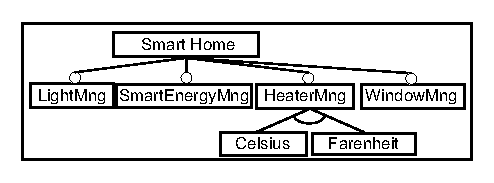
\includegraphics[width=.85\linewidth]{images/featureModel.eps} \\
    \caption{Smart Home feature model}
    \vspace{-15pt}
      \label{fig:SH-FM}
  \end{center}
\end{figure}

It specifies a Smart Home can optionally manage lights, windows and heaters. Moreover, there is a smart energy option which coordinates windows and heaters for save energy. For instance, before heating a room, if outside temperature is colder the software close the windows to avoid wasting energy. Obviously, this function required the heater and window function has been selected, which is specified by means of a required relationship.

Figure~\ref{fig:SH-DM} shows a UML model depicting a design supporting the variations specified for the previous feature model. Each coarse-grained feature, such as \imp{LightMng} is encapsulated in a UML package, as established by the feature-oriented design guidelines elaborated in the AMPLE project~\cite{sanchez:2007,nebrera:2008}. These packages are combined using UML merge relationships. UML merge relationships, roughly speaking, merge those elements of the same kind which match by name.
% Improve this
For instance, \imp{Gateway} classes will be merged to produce a combined version. Fine-grained variations are accommodated using other techniques, such as parametrization. So, variation in heaters measurement units is achieved by setting appropriately up an attribute in the \imp{HeaterCtrl} class.

%% Comment a little bit on the general arquitecture based on a gateway

\begin{figure*}[!tb]
  \begin{center}
  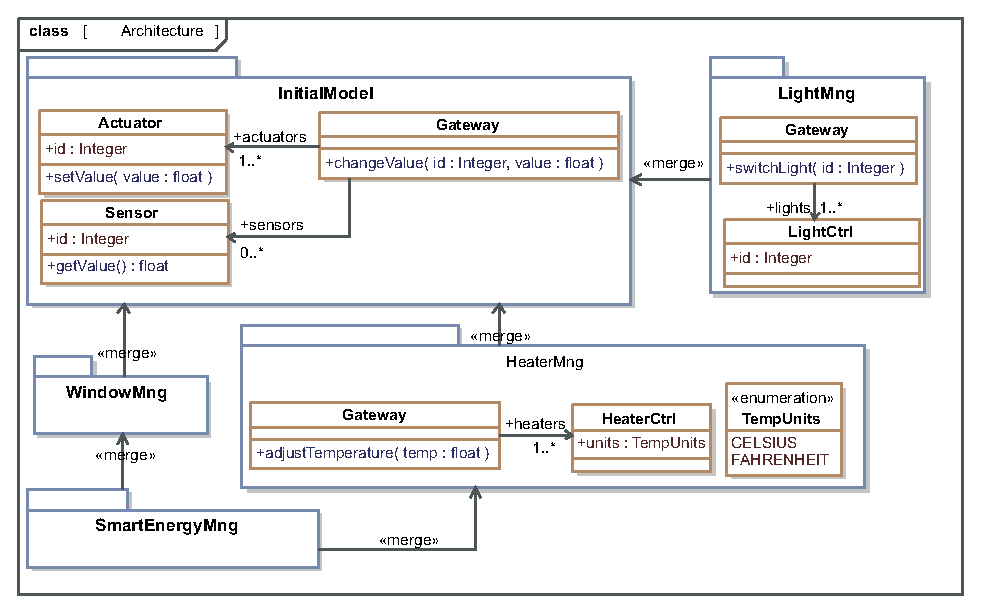
\includegraphics[width=\linewidth]{images/umlDesign.eps} \\
  \caption{Smart Home design}
  \label{fig:SH-DM}
  \end{center}
\end{figure*}

In the following sections, we will try to create an implementation of this feature-oriented design in C\# using partial classes. Strengthens and weaknesses of this technique will be identified.


\section{What we want to find in a feature-oriented programming language}
\label{sec:fopFeatures}

%=========================================================================%
% Author: Pablo S�nchez                                                   %
% Paper: FOSD2010 (FOP Features)                                          %
% Version: 1.0                                                            %
% Date   : 2010/05/07                                                     %
%=========================================================================%

This section describes which characteristics are desirable to find in a language to
support feature-oriented programming.

% Try to find better supporting references
Feature-Oriented Programming~\cite{prehofer:1997} aims to encapsulates coherent slices of the functionality provided by an application into independent and composable modules called \emph{features}. Therefore, different versions of a same application should be easily obtained by simply combining different set of features. Obviously, not all feature combinations lead to right final applications, so feature-oriented languages should try to ensure the result of composing a set of features produces a safe and correct application. For instance, for the previous

Wit these goals on mind, and based on~\cite{Herrejon:2005,kang:2002,chae:2009,aracic:2006}, we have identified several desirable characteristics we would like to find in a language for supporting feature-oriented programming. We comment on each one of them.

\paragraph{Feature Encapsulation and Extensibility}

A feature is often considered as an increment on program functionality~\cite{zave:1999,Herrejon:2005}. For instance, in the SmartHome case study, \imp{LightMng}, \imp{WindowMng}, and so forth, are increments on functionality for monitoring and controlling new devices. Thus, feature-oriented languages must provide mechanism for adding new functionality to the existing one. In object-oriented languages, extension is achieved by inheritance. Inheritance is adequate when we need to extend a single class, but commonly, features need to extend several classes at the same time. For instance, the \imp{LightMng} feature needs to add a new class for the light controller (\imp{LightCtrl}) and it needs to add to the \imp{Gateway} class methods for switching on and off lights. So, a language with feature-oriented support must provide extension mechanisms.

Extension is not always achieved by addition, sometimes \emph{substitution} is required. For instance, in the case of the \imp{SmartEnergyMng} feature, it is necessary, for instance, to override the implementation of the method \imp{adjustTemperature} for checking is additional operations are required. For instance, if the command is to cool a room with the windows closed and the outside temperature is lower than the indoor one, windows will be open in addition to switching off heaters. This kind of substitution is achieved in object-oriented languages by method overriding.

All the extensions belonging to a certain feature must be added in a atomic way, i.e. either all extensions are added or no extension is carried out at all. For instance, the \imp{Gateway} class must not be extended with the
\imp{swicthLight} method if the class \imp{Light} is not added at all. Therefore, featured-oriented languages should provide mechanisms to group and ideally encapsulate elements belonging to a same feature in well-identified modules. Moreover, these modules should be compilable separately. In Figure~\ref{fig:SH-DM}, we use UML packages with this purpose.

Finally, extensions might have unavoidable ripple effects. For instance, sensors might have a reference to the \imp{Gateway} class to send messages with urgent or critic situations are detected, such as fire, for instance. The class \imp{Gateway} is refined through each feature, thus, several versions of the \imp{Gateway} class are created, e.g. \imp{LightMng::Gateway}, \imp{HeaterMng::Gateway}, \imp{HeaterMng::Gateway} and so forth. Thus, depending upon the selected features the customer want to include in the final product, a specific subclass, or combination of subclasses, should be selected. Let us suppose we select the \imp{LightMng} feature. In that case, the version of the \imp{Gateway} to be included in the final product is \imp{LightMng::Gateway}. But, the \imp{Sensor} class references \imp{InitialModel::Gateway}. So, we should update constructors, getters, setters and so forth to reference the subclass, i.e. \imp{LightMng::Gateway}, and get rid of castings and other problems related to the type system. Usually, this need to be done manually. Nevertheless, some languages, such as CeasarJ~\cite{aracic:2006} or ObjectTeams~\cite{Herrmann:2007} are able to automatically update these dependencies due to the usage of an advanced type system based on virtual clases and mixin composition. So, automatic dependency management is also a desirable characteristic in feature-oriented languages.

\paragraph{Feature-Level Composition and Composition Consistency Checking}

Specific products, or configurations of a feature-oriented decomposition, are obtained by means of selecting a set of features. Thus, it would desirable a feature-oriented language would provide language constructs for specifying which specific features should be instantiated, or composed, when producing a specific product. This should be done at the feature-level, specifying which \emph{feature modules} should be included, instead of having to specify individual elements of each feature. For instance, if the \imp{LightMng} feature has been selected,
we would like to specify the \imp{LightMng} package should be included, according to Figure~\ref{fig:SH-DM}, instead of having to specify the \imp{LightMng::Gateway} feature and the \imp{LightCtrl} class must be added individually to the final product.

Moreover, neither all feature combinations can be composed safely nor all composition ordering are valid. For instance, if the \imp{SmartEnergyMng} feature is selected, the \imp{WindowMng} and \imp{HeaterMng} features should also be selected. Moreover, \imp{WindowMng} and \imp{HeaterMng} must be composed before \imp{SmartEnergyMng} is composed, since the latter one depends on the former ones. A feature-oriented language should be aware of these constraints, avoiding invalid product can be created and managing automatically dependencies whenever possible. For instance, when \imp{SmartEnergyMng} feature is selected, the language should detect the \imp{WindowMng} and \imp{HeaterMng} should be also composed and, in addition, before the \imp{SmartEnergyMng} feature.

So summarising, a feature-oriented language must provide:

\begin{enumerate}
    \item Feature Extension by addition and substitution.
    \item Modules to group and encapsulate feature elements.
    \item Automatic dependency management at intra-feature level.
    \item Composition at the feature level.
    \item Composition consistency checking.
    \item Automatic management of constraints at the feature level.
\end{enumerate}

Next section will evaluate how C\# partial classes are able to manage these issues. 

\section{Implementing the Smart Home models using C\# partial classes}
\label{sec:partialClasses}

This section describes the results of our experiment about using C\# partial classes to implement the feature-oriented design of the Smart Home case study. Before describing them, we provide some background on how C\# partial classes work.

\subsection{C\# partial classes}

%=========================================================================%
% Author : Alejandro P�rez Ruiz                                           %
% Author : Pablo S�nchez Barreiro                                         %
% Version: 1.1, 10/06/2011                                                %
% Master Thesis: Background/PartialClasses                                %
%=========================================================================%

Las clases parciales C\# \cite{albahari:2010} permiten dividir la implementaci�n de una clase en varios archivos de c�digo fuente. Cada fragmento representa una parte de la funcionalidad global de la clase. Todos estos fragmentos se combinan en tiempo de compilaci�n para crear una �nica clase, la cual contiene toda la funcionalidad especificada en las clases parciales. Por lo tanto, las clases parciales C\# parecen un mecanismo adecuado para implementar caracter�sticas, tal como ha sido identificado por diversos autores~\cite{laguna:2007,laguna:2010}, dado que cada incremento en funcionalidad perteneciente a una caracter�stica se podr�a encapsular en una clase parcial separada.

%%==============================================================================================================%%
%% NOTA(Pablo): Poner un ejemplo peque�o aqu� con dos clases parciales relativas al problema de las expresiones %%
%%==============================================================================================================%%

%%=============================================================================================================%%
%% NOTA(Pablo): Esto no me cuadra muy bien aqu�, as� que lo borro                                              %%
%%=============================================================================================================%%
%%
%% Para poder ser compiladas y agrupadas en una sola clase, todas las clases parciales deben pertenecer al
%% mismo espacio de nombres, poseer la misma visibilidad y deben ser declaradas con la palabra clave
%% \imp{partial}. En C\#, un espacio de nombre se emplea simplemente para agrupar clases relacionadas y evitar
%% conflictos de nombres.
%%
%%=============================================================================================================%%


Para especificar los archivos C\# que deben ser incluidos en una unidad de compilaci�n se emplea un documento XML como el de la Figura~\ref{back:fig:partialClass}. Por lo tanto, es posible incluir y excluir f�cilmente la funcionalidad encapsulada dentro de una clase parcial simplemente a�adiendo o eliminando dicha clase parcial de este fichero XML. Por tanto, la composici�n de caracter�sticas tambi�n parece factible mediante la manipulaci�n de este fichero XML.

\begin{figure}[!h]
\begin{center}
\begin{footnotesize}
\begin{verbatim}
01    <itemgroup>
02    <!--Eval-->
03    <Compile Include="Eval\Add.cs" />
04    <Compile Include="Eval\IExpressionsEval.cs" />
05    <Compile Include="Eval\IExpressions.cs" />
06    <Compile Include="Eval\Integer.cs" />
07    <Compile Include="Eval\Mult.cs" />
08    <!--Infix-->
09    <!--<Compile Include="Infix\Add.cs" />
10    <Compile Include="Infix\IExpressionInfix.cs" />
11    <Compile Include="Infix\IExpressions.cs" />
12    <Compile Include="Infix\Integer.cs" />
13    <Compile Include="Infix\Mult.cs" />-->
14    ...
15    </itemgroup>
16    </Project>
\end{verbatim}
\end{footnotesize}
\end{center}
\caption{Archivo XML que guarda la informaci�n para la compilaci�n en Visual Studio}
\label{back:fig:partialClass}
\end{figure}

%%=============================================================================================================%%
%% NOTA(Pablo): Esto no me cuadra muy bien aqu�, as� que lo borro                                              %%
%%=============================================================================================================%%
%% Para ilustrar lo dicho anteriormente, se ha vuelto a utilizar el problema de las expresiones implement�ndolo
%% con clases parciales. La figura \ref{back:fig:partialClass} muestra como hemos excluido de la compilaci�n la
%% caracter�stica que representa la operaci�n de imprimir una expresi�n en formato infijo.
%% Este mecanismo de clases parciales permite a�adir o compartir funcionalidad entre un conjunto de clases que
%% no precisan estar relacionadas mediante ning�n tipo de relaci�n jer�rquica, tal como ocurre con la herencia.



\subsection{Evaluation}

%=========================================================================%
% Author: Pablo S�nchez                                                   %
% Paper: FOSD2010 (Evaluation)                                            %
% Version: 1.0                                                            %
% Date   : 2010/07/20                                                     %
%=========================================================================%

\paragraph{Feature Encapsulation and Extensibility} \ \\

C\# partial classes does not seem to provide any mechanism to group an encapsulate features. We might use namespaces for this purpose. We might opt for placing all classes related to the \imp{InitialModel} and \imp{LightMng} features in the \imp{SmartHome.InitialModel} and \imp{SmartHome.LightMng} namespaces respectively. Nevertheless, in this case the \imp{Gateway} partial classes belonging to separate features will be not combined. Thus, partial classes force us to place all classes in a same namespace, so we can not use this mechanisms to group feature-related code.

Any other workaround, such as creating one coarse-grained class per feature and managing feature-specific classes as internal classes of the coarse-grained one will not work either, since the outer class serves as namespace for the internal classes. Thus, each internal class, although declared as partial, it is placed in a different namespace and they are not merge.

\begin{figure}
    \begin{center}
    \begin{small}
    \begin{verbatim}
File InitialModel/Gateway.cs
--------------------------------------------------------
01 public partial class Gateway {
02   ...
03   public Gateway() {
04     this.actuators = new List<Actuator>();
05     this.sensors = new List<Sensor>();
06   }
07 }
File LightMng/Gateway.cs
--------------------------------------------------------
08 public partial class Gateway {
09   protected List<LightCtrl> lights;
10   public Gateway() {
11       this.lights = new List<LightCtrl>();
12   }
13 }
    \end{verbatim}
    \end{small}
    \caption{\imp{Gateway} implementation using partial classes}
    \label{fig:constructor}
    \vspace{-15pt}
    \end{center}
\end{figure}

Regarding extensibility, partial classes allows us to add new attributes and methods to existing partial classes, but they do not allow us to extend or override existing ones. For instance, in the \imp{LightMng} feature, we have added a new attribute \imp{lights} to the \imp{Gateway} class. So, we should extend the \imp{Gateway} constructor to appropriately initialize this attribute. So, we write the code depicted in Figure~\ref{fig:constructor}. This excerpt of code contains the constructor for the most basic \imp{Gateway} class (Figure~\ref{fig:constructor}, lines 03-06), which is extended with new functionality in the \imp{LightMng} feature (Figure~\ref{fig:constructor}, lines 03-06). Nevertheless, this is not possible, since the compiler reports an error because the method \imp{Gateway()}, i.e. the class constructor, is duplicated. This means we can not split the implementation of a method into several files, since we can not have methods with the same signature into two separate files of a partial class. This reduces extensibility to the addition of new methods and attributes (as shown in Figure~\ref{fig:partialClass}), but we cannot add functionality to existing methods. It would be interesting if C\# supported \emph{partial methods} in addition to partial classes.

In the case of extensibility by substitution, the problem will be the same. Let us consider now the case of the \imp{SmartEnergyMng} feature. The \imp{Gateway} class for this feature must override, for instance, the \imp{adjustTemperature} method to check if additional operations involving the windows must be executed before adjusting the temperature. Nevertheless, since we can not declared a method \imp{adjustTemperature} in the partial class belonging to the \imp{SmartEnergyMng} feature with the signature as the method declared for the \imp{HeaterMng} feature, there is no way to override the latter one. Indeed, normal object-oriented overriding is somehow more complex than usual in C\# because, as in C++, for a method being effectively overridden, we need to declared it as \emph{virtual}. Thus, we need somehow to foresee a method is going to be overridden to declare it as virtual, or declare all methods as virtual, independently if we know they are going to be overridden or not. This last practice is the recommended one by authors, although it is tedious and verbose.

Regarding automatic management of dependencies between classes, C\# partial classes do not present the problem described in Section~\ref{sec:fopFeatures}. The problem was a class \imp{A}, e.g. \imp{Sensor} in Figure~\ref{fig:SH-DM}, has a reference to a class \imp{B}, e.g. \imp{Gateway}, which is refined by means of inheritance through different features. When a final product is created, this reference should be changed to the deepest child belonging to a selected feature in the inheritance tree to avoid castings and other problems related to the type system. This problem does not appear when using C\# partial classes because we are not using subclassing by inheritance. We are simply merging slices of the same class, so the type of a class is not changed although a class is refined through several features. Moreover, when a instance of a class, e.g. \imp{Gateway}, is created, this instance will be an instance of a class containing the functionality belonging to the all the selected features. So, regarding this particular point, C\# partial classes seems to provide a performance similar to languages such as CaesarJ or ObjectTeams.

\paragraph{Feature Level Composition} \ \\

Since they are not specific mechanisms to group and encapsulate a bundle of classes related to a same feature, it is not possible either to compose products at the feature level. Composition of specific products is achieved by means of including/excluding (partial) classes from the compilation unit, such as shown Figure~\ref{fig:partialClass}. This means we need to manage the elements belonging to a same feature individually, and take care of producing consistent configurations. For instance, we should check the \imp{LightCtrl} class is included in the compilation unit if and only if the partial class of \imp{Gateway} belonging to the \imp{LightMng} feature is also included. So, several actions must be carried out each time a feature is selected and deselected.

In the same way, C\# does not provide explicit mechanisms to guarantee a build file contains a valid selection of features. Nevertheless, if a feature uses classes and methods declared in another feature, the compiler will report an error about we are using some undefined elements. For instance, if the \imp{Gateway} partial class belonging to the \imp{SmartEnergyMng} feature use some classes called \imp{WindowCtrl} and \imp{HeaterCtrl} and we have not included them in the compilation unit, the compilation process will fail until we include these classes in the compilation unit. Nevertheless, we should not include only these classes, we should also include all the classes belonging to the \imp{LightMng} and \imp{HeaterMng} features. So, using C\# partial classes we can detect dependencies between classes, but not dependencies at the feature level, which would be the ideal case. If errors are detected, the compiler reports it, but it need to be solved manually, i.e. if the feature \imp{SmartEnergyMng} is included, the \imp{WindowMng} and \imp{HeaterMng} features need to be manually included. Finally, there is not support to detect and solve mutual exclusion constraints, i.e. situations where if a feature \imp{A} is selected, a feature \imp{B} must not be selected. Anyway, to the best of our knowledge, this kind of support is rarely found in feature-oriented languages.  

\subsection{Conclusions}

%=========================================================================%
% Author: Pablo S�nchez                                                   %
% Paper: FOSD2010 (Discussion)                                            %
% Version: 1.0                                                            %
% Date   : 2010/07/20                                                     %
%=========================================================================%

According to the results shown in previous section, we must conclude C\# partial classes are not a suitable mechanism to achieve feature-oriented programming. The main problems come from:

\begin{enumerate}
    \item Lack of support for feature modules and feature encapsulation.
    \item Lack of support for extending existing methods.
    \item Lack of support for overriding existing methods.
    \item Lack of support for composition at the feature level.
\end{enumerate} 

%\section{Sketch of solutions for C\# partial classes pitfalls}
%
%Breves comentarios sobre como solucionar estos problemas. (NOTA: No estoy muy seguro acerca de si poner o no esta secci�n).

\section{Summary and Future Work}
%=========================================================================%
% Author: Pablo S�nchez                                                   %
% Paper: FOSD2010 (Sumary And Future Work)                                %
% Version: 1.0                                                            %
% Date   : 2010/07/25                                                     %
%=========================================================================%

\paragraph{Sumary} \ \\

This work has evaluated the characteristics that should ideally be supported in a feature-oriented programming language. It proposes the following:

\begin{enumerate}
\item The feature-oriented languages should provide mechanisms to group and encapsulate those elements that integrate a characteristic in order to facilitate other elements such as the capacity for extension and refinement of features. This type of language should take into account some form of adding new functionalities to the existing ones. For example, LightMng and HeaterMng are extensions of functionality for controlling and monitoring new devices. At the same time, on certain occasions it is also necessary to rely on a sufficiently-flexible mechanism of substitution. For instance, in the case of the feature SmartEnergyMng, it is necessary to override the method implementation adjustTemperature in order to verify if it is necessary to perform additional operations according to the data collected by sensors.

\item Ideally, a feature-oriented language should provide constructions at level of features in order to specify which features should be instantiated or composed to produce a specific product. It should identify which modules should be included rather than having to specify the individual elements of each feature. Moreover, all of the included feature combinations should make up a secure and valid entity. For instance, if the feature SmartEnergyMng is selected, the features HeaterMng and WindowMng should implicitly be selected and composed before. This is known as composition and checking of features. 

\item This project has evaluated the utilization of partial classes C\# for feature-oriented implementations providing critical point of view thereof. In order to do so, it has employed the SmartHome case study as model to specify elements belonging to a software product-line and manage of variability. This evaluation has determined, in the first case, that the partial classes lack a grouping mechanism for encapsulating features. As such, it is not possible to compose products at the level of features as is described in section 4.3. With regard to the extensibility capacity, the partial classes allow us to add new attributes and methods to the existing partial classes; however, they do not allow us to extend or replace those that already exist. For this reason, the capacity to substitute elements is limited. Another aspect is that C\# lacks a mechanism that allows for the automatic composition of dependencies, which would allow referencing the most specialised classes in a feature-selection for a specific product.
\end{enumerate} 

\paragraph{Future Work} \ \\

As future work to undertake, would be to perform the necessary task such that partial classes provide a flexible and consistent manner of feature-oriented implementation, which could be to extend the C\# language in an optimal way that includes the following recommendations:

\begin{enumerate}
\item Provide an additional encapsulation unit that groups the classes contained in the features, such that can be compose products from this level. It would take into account the restrictions and the ideal consistency of the model for each included class.
\item Introduce a refining mechanism that supports overwriting methods defined in partial classes contained in distinct features without inheritance neither virtual methods declaration. 

\item Solve the manual rebinding of dependencies, automatically updating constructors and other methods to make reference to the sub-class, dependent upon the characteristics included in the final product. 

\item Provide checking of consistency of the compositions at the feature level.
\end{enumerate} 

Currently MS. Visual Studio .Net has at users disposal, tools for creating its own extensions .Net. The index of utilities is called Automization Model. By means of this index, it is possible to extend the basic functionality of IDE with certain tools directed principally at the creation of add-ins, macros and program integrations attachable to the environment of development. For this reason, part of the future work will also be to investigate the scope of these tools and to evaluate the appropriate way for which to implement the relevant extensions. 




\label{sec:summary}

\bibliographystyle{plain}
\bibliography{fosd2010}

\balancecolumns

\end{document}
